%\vspace{-1ex}
\section{Introduction}
\label{sec:intro}


% reachability query application
There is a wide range of emerging applications of
graph-structured data, {\it e.g.}, bioinformatics, communication
networks, social networks, web topology and semi-structured data. Many graph queries have been proposed to retrieve such graph
data.
%%
% problem of management of data and query
%%
% Byron: in reality, graphs are not managed by users.
However, as the volume of graph data is increasing at an unprecedented rate,
hosting efficient query services has become a technically challenging task.  The
{\em owners} of graph data may not always be equipped with the expertise
required to provide such services and therefore may
%%
% query services
%%
employ {\em query service providers} (\SP s) to host {\em query services}, which
are often supported by high performance computing. Security (such as
the confidentiality of messages exchanged) has been stated as one of the
attributes of Quality of Services (QoS) \cite{issues}, as \SP\ s cannot always be
trusted. This attribute may influence the willingness of both data owners and query clients to use \SP's services.


% motivate the query together with privacy
Take the reachability query ---  one of the most fundamental and popular graph queries
\cite{cohen, ferrari, sigmod2012, grail, gripp, 3hop, pathhop, hopi, chengjf1,
chengjf2, byron, cikmlabel, bitcompression, pathtree} --- as an example:  {\em
Given two nodes $u$ and $v$ of a graph, the reachability query is used to test if $v$
is reachable from $u$ or not}.
% privacy problem of employment of query services 
A query client may prefer not to expose his/her reachability query to an \SP.
On the other hand, the data owner may prefer that the \SP\ not be able to infer
the structure of their graph data. Therefore, the query results must be
protected as malicious \SP s can exploit the results from multiple queries to
infer the graphs' structures.



\stab
\noindent {\bf Motivating example.} Consider a pharmaceutical company
whose revenue depends mostly on the invention of Health Care Products,
illustrated in Fig.~\ref{fig:overview}. The company may have
discovered new compounds for a new product. To save laboratory
experiments, it may query the compounds from web-accessible biological
pathway networks (such as \cite{biology}) to understand the compounds'
characteristics, such as whether it is possible for the compounds to
form other compounds via any chemical reactions (reachability in the
network). However, on the one hand, the company does not want the
\SP\ to know about the queries (the compounds), as it may apply for
patents for the synthesis. On the other hand, the owner of the pathway
networks may not only lack the experience to host query services but
also be reluctant to release the networks to the public.
Alternatively, the owner is willing to release a license only to paid
users.  Therefore, it is crucial to protect {\em both} the queries and
the network from the \SP.



\begin{figure}[t]
\begin{minipage}[t]{0.5\linewidth}
\centering
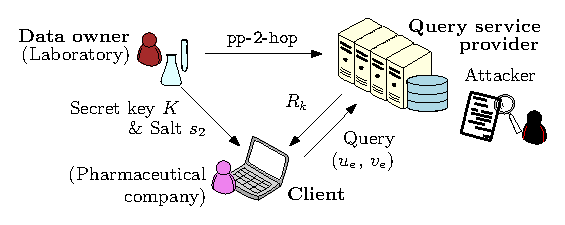
\includegraphics[width=2.2in]{./example/system.eps}
\vspace{-2ex}
\caption{Overview of the system model}
\label{fig:overview}
\end{minipage}%
\begin{minipage}[t]{0.5\linewidth}
\centering
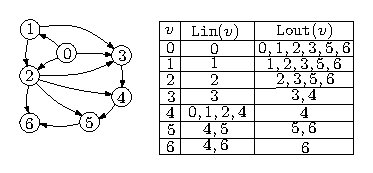
\includegraphics[width=1.6in]{./example/graph.eps}
\vspace{-4ex}
\caption{A (partial) schematic of a biological network  (LHS) and its \hop\ labeling (RHS)}
\label{fig:2hop}
\end{minipage}
%\vspace{-6ex}
\end{figure}

\stab
% Problem statement
This paper studies the problem of {\em evaluating the reachability
  query at an \SP\ without compromising the privacy of the
  reachability of the query nodes and the graph structure under
  cipertext-only and size-based attacks, in the paradigm of query
  services} (to be detailed with Fig.~\ref{fig:overview} in
Sec.~\ref{sec:preliminary}). To our knowledge, this has not been  addressed before.



% related reachability works in the literature (in light of privacy preservation)
There have been many recent studies  on efficient reachability query ({\it
e.g.}, \cite{pathtree, bitcompression,grail, gripp, ferrari,3hop, pathhop,
sigmod2013, hopi, chengjf1 ,chengjf2, byron}). Jin et al. \cite{sigmod2012}
show that these studies can be roughly categorized into {\em transitive closure
compressions}, {\em refined online search} and {\em hop labeling}. The first
two categories suffer from high storage costs and require
online searches, respectively (to be discussed in
Sec~\ref{subsec:related:reach}).
% adopt and motivate 2hop
In this paper, we propose our techniques based on hop  labeling
\cite{cohen}, in particular \hop\ labeling. The benefits of adopting \hop\ labeling are
threefold. Firstly, the structures of \hop\ labels are simple, where
each node is associated with two sets of nodes called $\lin$ and
$\lout$. Secondly, the query evaluation with \hop\ labeling is
an intersection between an $\lin$ and an $\lout$. Such simple
structure and algorithm make privacy
preservation plausible. Thirdly, \hop\ labeling is an active research
topic. The recent works on large graph  partitioning ({\it e.g.}, \cite{chengjf2}),
compression ({\it e.g.}, \cite{chengjf1}) and maintenance ({\it e.g.},
\cite{hopi,byron}) of \hop\ labeling can be readily adopted.




% the challenges and our solutions
% Byron: your methodologies
% addition of surrogate nodes
This paper proposes \pphop\ ({\em privacy preserving \hop}), which adopts
\hop\ labeling. 
%%%%
Firstly, 
the evaluation of each query on \hop\ labeling only involves an intersection between
two sets of center nodes.  Hence, we minimize the size of the
maximum cardinality of the intersection results and add {\em minimal}
artificial nodes (called surrogate nodes) to $\lin$s and $\lout$s such
that the intersection results for all possible queries are of the {\em
  same} size. We  unify each of the $\lin$ and $\lout$
labels such that the difference of the label set sizes are
within a user-defined parameter.
%%%%
Secondly, we encrypt the \hop\ labels, after adding surrogate nodes
and evaluate queries in the encrypted domain. We analyze the privacy
of \pphop.
% encryption of the index optimization
\eat{For optimization, we propose a heuristic function to minimize the maximum
cardinality of the intersection during query evaluation. }



% contribution
\noindent The contributions of this paper are summarized as follows.
\vspace{-1ex}
\begin{itemize}%\addtolength{\itemsep}{-0.3\baselineskip}

        \item We propose algorithms to  unify the sizes of \hop\ labels and the
            query result sizes; \eat{realize minimum addition
            of the surrogate nodes in 2-hop labeling;}

        \item We propose private query
            processing over the  encrypted \hop\ labels;

        \item We propose  a new heuristic \hop\ construction that yields \hop\
            labeling that minimizes the intermediate results in private query
            processing; and

        \item We conduct an empirical study to confirm that our techniques are efficient.
\end{itemize}
\vspace{-1ex}

The rest of this paper is organized as follows. We
introduce some related work in Sec.~\ref{sec:related}. We then present the
background, the problem and the overview of our solution in Sec.~\ref{sec:preliminary}. We
propose \pphop, the index construction, optimization  and query processing in
Sec.~\ref{sec:preprocessing}. We conduct a  privacy analysis in
Sec.~\ref{sec:analysis}. We present an experimental evaluation in
Sec.~\ref{sec:exp}. We end this paper with the conclusion in
Sec.~\ref{sec:conclusion}.





















